\documentclass{beamer}
\usetheme{Boadilla}

\usepackage{amsmath}
\usepackage{amsfonts}
\usepackage{hyperref}



\title{Gumbel distribution}
\author{Skorik Sergey}
\institute{MIPT, 2022}


\begin{document}

\begin{frame}
    \titlepage
\end{frame}


\begin{frame}
    \tableofcontents
\end{frame}


\section{Definition and properties}

\begin{frame}{Definition and properties}
    \begin{block}{Definition}
    Let $\xi \sim Gumbel(\mu, \beta)$, then
    \begin{equation}
        \label{gumbel_pdf}
        f_{\xi}(x) = \dfrac{1}{\beta}\exp{\left(-\dfrac{x - \mu}{\beta} + \exp{\left[\dfrac{x - \mu}{\beta}\right]}\right)}, \quad x, \mu \in \mathbb{R}, \beta \in \mathbb{R}_+
    \end{equation}
    Also cumulative distribution function of the Gumbel distribution is
    \begin{equation}
        \label{gumbel_cdf}
        F_\xi(x) = \int\limits_{-\infty}^x \dfrac{1}{\beta}\exp{\left(-\dfrac{t - \mu}{\beta} + \exp{\left[\dfrac{t - \mu}{\beta}\right]}\right)}dt = \exp\left\{-\exp{\left(-\dfrac{x - \mu}{\beta}\right)}\right\}
    \end{equation}
    \end{block}

\end{frame}

\begin{frame}{Definition and properties}
    \begin{figure}[h]
\caption{Cumulative distribution function}
\centering
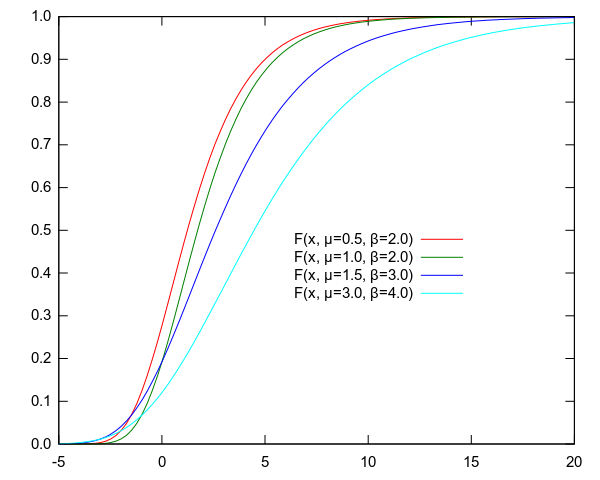
\includegraphics[width=10cm, height=7cm]{Gumbel-Cumulative.png}
\end{figure}

\end{frame}


\begin{frame}{Definition and properties}
        \begin{figure}[h]
\caption{Probability density function}
\centering
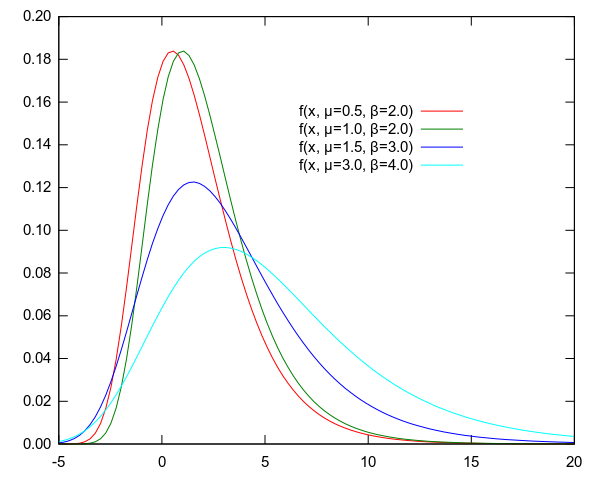
\includegraphics[width=10cm, height=7cm]{Gumbel-Density.png}
\end{figure}
\end{frame}


\begin{frame}{Definition and properties}
    \begin{block}{Properties}
        Let $\xi \sim Gumbel(\mu, \beta)$, then
        \begin{itemize}
            \item \[\mathbb{E}[\xi] = \mu + \beta\gamma\]
            where $\gamma = \lim\limits_{n\to\infty}\left(-\log n + \sum_{k=1}^n\dfrac{1}{k}\right)$ is  Euler–Mascheroni constant
            \item \[\mathbb{D}[\xi] = \dfrac{\pi^2}{6}\beta\]
            \item \[Q(p) = \mu - \beta\log(-\log p ), \quad 0 < p < 1\]
        \end{itemize}
    \end{block}
\end{frame}

\section{Applications}
\begin{frame}{Applications}
    \begin{block}{Extreme value theory}
        Gumbel distribution is I-type of generalized extreme value distribution, which is used to model the distribution of the maximum (or the minimum) of a number of samples of various distributions. 

        Let $X_1, \ldots X_n$ be a sequence of i.i.d random variables with CDF $F$ and let $M_n = \max{(X_1, \ldots X_n)}$. Note, that
        \[\Pr(M_n \leq z)  = \Pr(X_1 \leq z, \dots, X_n \leq z)\]
        \[ = \Pr(X_1 \leq z) \cdots \Pr(X_n \leq z) = (F(z))^n\]
        The associated indicator function $I_n = I(M_n > z)$ is a Bernoulli process with a success probability $p(z) = 1 - (F(z))^n$
    \end{block}
\end{frame}

\begin{frame}{Applications}
    \begin{block}{Extreme value theory}
        In practice, we might not have the distribution function $F$. 

        \textit{Fisher–Tippett–Gnedenko theorem:}  If there exist sequences of constants $a_{n}>0$ and $b_n \in \mathbb{R}$ such that
        \[\mathbb{P}\left[\dfrac{M_n - b_n}{a_n}\leq z\right] \underset{n\to\infty}{\longrightarrow} G(z)\]
        then
        \[G(z) \propto \exp{\left[-(1 + \zeta z)^{-1/\zeta}\right]}\]
        In case when $M_n$ has an exponential tail
        \[G(z) = \exp\left\{-\exp{\left(-\dfrac{z - b}{a}\right)}\right\}\]
        Is a gumbel CDF. 
    \end{block}
\end{frame}

\begin{frame}{Applications}
    Let's consider application to extreme rainfall data\footnote{\textbf{A Bayesian analysis of the Gumbel distribution: an application to extreme rainfall data}; https://link.springer.com/article/10.1007/s00477-013-0773-3}
    \begin{block}{Application to extreme rainfall data}
        Let $I(t)$ be the rainfall intensity in the time $t$, then the quantity $Y_k(d) = \int\limits_{k}^{k+d}I(t)dt$ is observed. $Y_{ijk}(60)$ the k-th quantity in a year $i$ in day $j$ for the period $d = 60$ minutes. Then, for the $i$-th year it is reported that $M_i(d) = \max_{j, k}\{Y_{ijk}(d)\}$ would be the annual maximum rainfall for duration $d$.

        The assumption then $Y_{ijk}(d)$ are i.i.d. random variables of a distribution with tails that fall exponentially gives by Fisher–Tippett–Gnedenko theorem that $M_1, \ldots M_n \overset{i.i.d}{\sim} Gumbel(\mu, \beta)$. So, the prior distribution
        \[f_{\xi}(x) = \dfrac{1}{\beta}\exp{\left(-\dfrac{x - \mu}{\beta} + \exp{\left[\dfrac{x - \mu}{\beta}\right]}\right)}\]
    \end{block}
\end{frame}

\begin{frame}{Gumbel Trick}
    \begin{block}{Gumbel Trick}
        Consider "log-sum-exp" quantities
        \[\log\left(\sum_{i=1}^n\exp{x_i}\right)\]
        They often used in optimization, they are a standard way of performing a soft maximum. In this context, the function defined as
        \[f_{\varepsilon}(x) = \varepsilon \log\left(\sum_{i=1}^n\exp{\frac{x_i}{\varepsilon}}\right) \Rightarrow \lim\limits_{\varepsilon\to 0^+}f_\varepsilon (x) = \max\{x_1, \ldots x_n\}\]
        Is it possible to go from the maximum back to the softmax $f_\varepsilon (x)$ ?
    \end{block}
\end{frame}

\begin{frame}{Gumbel Trick}
    \begin{block}{Gumbel Trick}
        The Gumbel trick provides a surprising randomized solution. Let $\gamma_1, \ldots \gamma_n$ be the i.i.d. random variables. Reparametrize vector $x_i \in \mathbb{R}^n$
        \[y = x + \gamma, \quad z = \max\{y_1, \ldots y_n\} = \max\{x_1 + \gamma_1, \ldots x_n + \gamma_n\}\]
        The trick is that by choosing $\gamma_1, \ldots, \gamma_n \sim Gumbel(\mu, \beta)$ we get
        \[\mathbb{E}z = \mathbb{E}[\max\{x_1 + \gamma_1, \ldots x_n + \gamma_n\}] = \log\left(\sum_{i=1}^n\exp{x_i}\right)\]
    \end{block}
    
    \begin{block}{Application in machine learning}
        The Gumbel trick can be used in mainly two ways: (a) the main goal is to approximate the expectation using a finite average or using stochastic gradients (then only the value of the maximum is used), (b) the minimizer is used for sampling purposes.
    \end{block}
\end{frame}

\end{document}
